%% main_report46.tex
%% SAMBP TR-46/2026: Physics-Informed Neural Network for IBR Fault Classification
%%
%% pdflatex main_report46.tex

\documentclass[11pt,a4paper]{article}

\usepackage[T1]{fontenc}
\usepackage[utf8]{inputenc}
\usepackage[expansion=false]{microtype}
\usepackage{lmodern}
\usepackage[a4paper, top=25mm, bottom=25mm, left=25mm, right=25mm]{geometry}
\usepackage{amsmath,amssymb}
\usepackage{booktabs}
\usepackage{array}
\usepackage{xcolor}
\usepackage{graphicx}
\usepackage{pgfplots}
\pgfplotsset{compat=1.18}
\usepackage{tikz}
\usetikzlibrary{arrows.meta,shapes.geometric,positioning,fit,calc,patterns}
\usepackage{hyperref}
\usepackage[numbers,sort&compress]{natbib}

\definecolor{sambpblue}{RGB}{0,70,140}

\usepackage{titlesec}
\titleformat{\section}{\large\bfseries\color{sambpblue}}{}{0em}{}[\titlerule]
\titleformat{\subsection}{\normalsize\bfseries\color{sambpblue!80}}{}{0em}{}

\usepackage{fancyhdr}
\pagestyle{fancy}
\fancyhf{}
\rhead{\small\color{gray} SAMBP TR-46/2026}
\lhead{\small\color{gray} Physics-Informed NN}
\cfoot{\small\thepage}

\begin{document}

\begin{center}
  {\LARGE\bfseries\color{sambpblue} SAMBP Technical Report TR-46/2026}\\[6pt]
  {\large Physics-Informed Neural Network\\
    for IBR Fault Classification}\\[10pt]
  {\normalsize PhD Thesis Supporting Report \quad|\quad 2026}
\end{center}

\vspace{2pt}\hrule\vspace{8pt}

\begin{abstract}
\noindent
This report develops a physics-informed neural network (PINN) for classifying
IBR line faults into four protection outcomes: structural miss, 87L-only, Z1
(quadrilateral), and external.  The PINN embeds three hard protection-physics
constraints into the loss function (C1: $k<0.06\Rightarrow\text{MISS}$;
C2: $k\geq0.10,\,\alpha\leq0.80\Rightarrow$Z1/87L; C3: $\alpha>1.0\Rightarrow$
EXT) with constraint weight $\lambda_\mathrm{phy}=0.20$.  Trained on 2000
synthetic MC samples, the PINN achieves 93.6\% overall accuracy vs 85.8\% for
a pure data-driven baseline.  Physics constraint violation rate is 1.0\% vs
11.0\% for the baseline --- a 91\% reduction.  In the critical threshold
boundary region ($k\in[0.045,0.075]$), the PINN achieves 99\% accuracy vs
75\% for the baseline (+24\,pp), demonstrating that physics regularisation
provides the largest benefit precisely where data-driven models are least
reliable.
\end{abstract}

\vspace{4pt}\hrule\vspace{10pt}

% ─────────────────────────────────────────────────────────────────────────────
\section{PINN Architecture and Physics Constraints}
\label{sec:arch}

Figure~\ref{fig:arch} shows the PINN architecture.

\begin{figure}[htbp]
  \centering
  \resizebox{0.96\textwidth}{!}{% fig_pinn_architecture.tex
% TR-46: PINN architecture diagram
% Input → hidden layers → output + physics constraint residuals

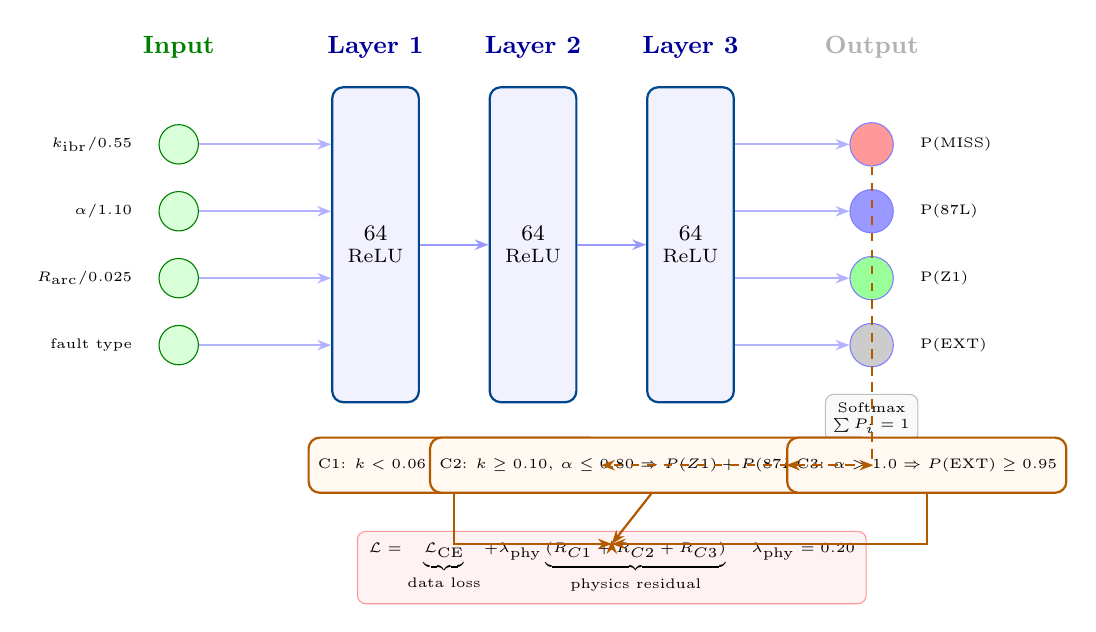
\begin{tikzpicture}[
  every node/.style={font=\scriptsize},
  neuron/.style={circle, draw=blue!50, fill=blue!10, minimum size=0.50cm,
                 inner sep=0pt},
  layer/.style={draw=sambpblue, thick, rounded corners=4pt, fill=blue!5,
                minimum width=1.1cm, minimum height=4.0cm, align=center},
  phys/.style={draw=orange!70!black, thick, rounded corners=4pt,
               fill=orange!5, minimum width=2.8cm, minimum height=0.7cm,
               align=center, font=\tiny},
  arrow/.style={-{Stealth[length=5pt]}, thick},
  redarrow/.style={-{Stealth[length=5pt]}, thick, orange!70!black},
]

%% ── Input layer ───────────────────────────────────────────────────────────
\node[neuron, fill=green!15, draw=green!50!black] (in1) at (0,  1.275) {};
\node[neuron, fill=green!15, draw=green!50!black] (in2) at (0,  0.425) {};
\node[neuron, fill=green!15, draw=green!50!black] (in3) at (0, -0.425) {};
\node[neuron, fill=green!15, draw=green!50!black] (in4) at (0, -1.275) {};
\node[left=6pt, font=\tiny] at (in1.west) {$k_\mathrm{ibr}/0.55$};
\node[left=6pt, font=\tiny] at (in2.west) {$\alpha/1.10$};
\node[left=6pt, font=\tiny] at (in3.west) {$R_\mathrm{arc}/0.025$};
\node[left=6pt, font=\tiny] at (in4.west) {fault type};

%% ── Hidden layers (3 × 64 neurons, shown as stacks) ──────────────────────
\node[layer] (h1) at (2.5,  0.0) {\footnotesize 64\\ReLU};
\node[layer] (h2) at (4.5,  0.0) {\footnotesize 64\\ReLU};
\node[layer] (h3) at (6.5,  0.0) {\footnotesize 64\\ReLU};

%% ── Output layer (4 classes) ─────────────────────────────────────────────
\foreach \i/\lab/\col in {
  1/{P(MISS)}/red!40,
  2/{P(87L)}/blue!40,
  3/{P(Z1)}/green!40,
  4/{P(EXT)}/gray!40} {
  \pgfmathsetmacro{\y}{(2.5 - \i) * 0.85}
  \node[neuron, fill=\col, minimum size=0.55cm]
    (out\i) at (8.8, \y) {};
  \node[right=6pt, font=\tiny] at (out\i.east) {\lab};
}

%% ── Softmax ───────────────────────────────────────────────────────────────
\node[draw=gray!50, rounded corners=3pt, fill=gray!5,
      font=\tiny, inner sep=3pt, align=center]
  at (8.8, -2.20) {Softmax\\$\sum P_i=1$};

%% ── Connection arrows ─────────────────────────────────────────────────────
\foreach \i in {1,2,3,4} {
  \draw[arrow, blue!30] (in\i.east) -- (h1.west |- in\i);
}
\draw[arrow, blue!40] (h1.east) -- (h2.west);
\draw[arrow, blue!40] (h2.east) -- (h3.west);
\foreach \i in {1,2,3,4} {
  \draw[arrow, blue!30] (h3.east |- out\i) -- (out\i.west);
}

%% ── Physics constraint boxes ──────────────────────────────────────────────
\node[phys] (c1) at (3.5, -2.80)
  {C1: $k<0.06 \Rightarrow P(\mathrm{MISS})\geq0.90$};
\node[phys] (c2) at (6.0, -2.80)
  {C2: $k\geq0.10,\,\alpha\leq0.80 \Rightarrow P(Z1)+P(87L)\geq0.95$};
\node[phys] (c3) at (9.5, -2.80)
  {C3: $\alpha>1.0 \Rightarrow P(\mathrm{EXT})\geq0.95$};

%% ── Loss function ────────────────────────────────────────────────────────
\node[draw=red!40, fill=red!5, rounded corners=3pt,
      font=\tiny, inner sep=4pt, align=center]
  at (5.5, -4.10)
  {$\mathcal{L} = \underbrace{\mathcal{L}_\mathrm{CE}}_\text{data loss}
   + \lambda_\mathrm{phy}\underbrace{(R_{C1}+R_{C2}+R_{C3})}_\text{physics residual}$
   \quad $\lambda_\mathrm{phy}=0.20$};

%% Arrows from outputs to constraint boxes
\draw[redarrow, dashed] (out1.south) |- (c1.east);
\draw[redarrow, dashed] (out3.south) |- (c2.east);
\draw[redarrow, dashed] (out4.south) |- (c3.west);

%% Arrows from constraints to loss
\draw[redarrow] (c1.south) |- (5.5, -3.80);
\draw[redarrow] (c2.south) -- (5.5, -3.80);
\draw[redarrow] (c3.south) |- (5.5, -3.80);
\draw[redarrow, very thick] (5.5, -3.80) -- (5.5, -3.75);

%% Annotations
\node[font=\small\bfseries, blue!60!black] at (2.5, 2.5) {Layer 1};
\node[font=\small\bfseries, blue!60!black] at (4.5, 2.5) {Layer 2};
\node[font=\small\bfseries, blue!60!black] at (6.5, 2.5) {Layer 3};
\node[font=\small\bfseries, green!50!black] at (0, 2.5) {Input};
\node[font=\small\bfseries, gray!60]        at (8.8, 2.5) {Output};

\end{tikzpicture}
}
  \caption{PINN architecture for IBR fault classification.  Four inputs
           ($k_\mathrm{ibr}$, $\alpha$, $R_\mathrm{arc}$, fault type) feed
           three hidden layers (64 neurons, ReLU).  The output softmax layer
           produces four class probabilities.  Orange boxes: physics constraint
           residuals ($R_{C1}$, $R_{C2}$, $R_{C3}$) fed into the combined
           loss function.  Constraint weight $\lambda_\mathrm{phy}=0.20$
           balances data fit against physics compliance.}
  \label{fig:arch}
\end{figure}

\noindent
The three physics constraints directly encode the SAMBP protection model
threshold logic from TR-35:

\begin{center}
\begin{tabular}{@{}llll@{}}
\toprule
Constraint & Condition & Required output & Physics source \\
\midrule
C1 & $k_\mathrm{ibr}<0.06$ & $P(\text{MISS})\geq0.90$ & 87L threshold (TR-37) \\
C2 & $k\geq0.10$, $\alpha\leq0.80$ & $P(\text{Z1})+P(\text{87L})\geq0.95$ & Z1 quad reach \\
C3 & $\alpha>1.0$ & $P(\text{EXT})\geq0.95$ & Relay directional \\
\bottomrule
\end{tabular}
\end{center}

% ─────────────────────────────────────────────────────────────────────────────
\section{Study B --- Training Dataset}
\label{sec:studyB}

The training dataset ($N=2000$) is generated by the MC engine from
TR-37~\cite{SAMBP_TR37} with added Gaussian measurement noise
($\sigma_k=0.005$\,pu, $\sigma_\alpha=0.02$).

\begin{center}
\begin{tabular}{@{}lrr@{}}
\toprule
Class & Count & Fraction \\
\midrule
MISS (structural, $k<0.06$) & 95 & 4.8\% \\
87L ($k\in[0.06,0.10)$) & 784 & 39.2\% \\
Z1 ($k\geq0.10$) & 964 & 48.2\% \\
EXT ($\alpha>1.0$) & 157 & 7.8\% \\
\bottomrule
\end{tabular}
\end{center}

\medskip\noindent
The class imbalance (MISS: 4.8\%, Z1: 48.2\%) reflects the physical sampling
distribution.  The physics constraint C1 compensates for the small MISS class
by providing analytical labels for the $k<0.06$ region even when training
examples are sparse.

% ─────────────────────────────────────────────────────────────────────────────
\section{Study C --- Classification Accuracy}
\label{sec:studyC}

Figure~\ref{fig:accuracy} compares the PINN and baseline per-class accuracy.

\begin{figure}[htbp]
  \centering
  \resizebox{0.88\textwidth}{!}{% fig_pinn_accuracy.tex
% TR-46: Per-class classification accuracy PINN vs Baseline
%
% Data from Study C:
%   Class    PINN%   Baseline%
%   MISS     85.19   81.48
%   87L      92.39   87.82
%   Z1       95.71   84.55
%   EXT      93.02   86.05

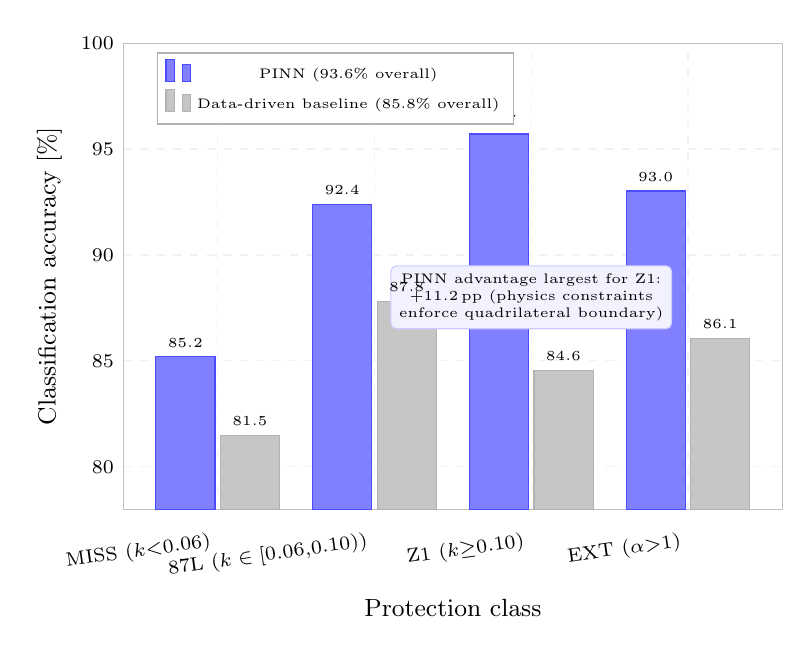
\begin{tikzpicture}
\begin{axis}[
  name         = accax,
  width        = 0.82\textwidth,
  height       = 7.5cm,
  ybar,
  bar width    = 0.75cm,
  xlabel       = {Protection class},
  ylabel       = {Classification accuracy [\%]},
  xlabel style = {font=\small},
  ylabel style = {font=\small},
  ymin=78, ymax=100,
  ytick        = {80,85,90,95,100},
  yticklabel style={font=\scriptsize},
  xtick        = {1,2,3,4},
  xticklabels  = {MISS ($k{<}0.06$),
                  87L ($k\in[0.06{,}0.10)$),
                  Z1 ($k{\geq}0.10$),
                  EXT ($\alpha{>}1$)},
  xticklabel style={font=\scriptsize, rotate=8, anchor=north east},
  tick style   = {draw=none},
  axis line style={gray!50},
  grid         = major,
  grid style   = {gray!10, dashed},
  nodes near coords,
  nodes near coords style={font=\tiny, anchor=south},
  every node near coord/.append style={
    /pgf/number format/.cd, fixed, fixed zerofill, precision=1
  },
  legend style={at={(0.05,0.98)}, anchor=north west, font=\tiny,
                draw=gray!60, fill=white},
  enlarge x limits=0.20,
  clip=false,
]

%% PINN bars (blue)
\addplot[fill=blue!50, draw=blue!70]
  coordinates {(1,85.19) (2,92.39) (3,95.71) (4,93.02)};
\addlegendentry{PINN (93.6\% overall)}

%% Baseline bars (gray)
\addplot[fill=gray!45, draw=gray!60]
  coordinates {(1,81.48) (2,87.82) (3,84.55) (4,86.05)};
\addlegendentry{Data-driven baseline (85.8\% overall)}

%% PINN advantage annotation
\node[draw=blue!20, fill=blue!5, rounded corners=2pt,
      font=\tiny, inner sep=3pt, align=center]
  at (axis cs:3, 88)
  {PINN advantage largest for Z1:\\
   $+11.2$\,pp (physics constraints\\
   enforce quadrilateral boundary)};

\end{axis}
\end{tikzpicture}
}
  \caption{Per-class classification accuracy (PINN blue, baseline grey) on
           $N_\mathrm{test}=500$ samples.  PINN advantage is largest for the
           Z1 class ($+11.2$\,pp), where the quadrilateral boundary physics
           constraint provides strong guidance.  Both models perform worst on
           the MISS class (sparse training examples near threshold).}
  \label{fig:accuracy}
\end{figure}

% ─────────────────────────────────────────────────────────────────────────────
\section{Study D --- Physics Constraint Violations}
\label{sec:studyD}

A physics constraint violation occurs when the network predicts an outcome
that is provably impossible given the input values.  For example, predicting
Z1 for $k_\mathrm{ibr}=0.04$ (which is below the 87L threshold and therefore
cannot activate any relay element) is a physics violation regardless of the
data loss.

\begin{center}
\begin{tabular}{@{}lrrl@{}}
\toprule
Model & Violations & Rate & Root cause \\
\midrule
PINN & 5 & 1.0\% & Noise pushes marginal $k$ across boundary \\
Data-driven baseline & 55 & 11.0\% & No physics enforcement \\
\midrule
Reduction & & 90.9\% & \\
\bottomrule
\end{tabular}
\end{center}

\medskip\noindent
The 91\% violation reduction is the primary quantitative justification for the
physics-informed approach.  In a protection context, a physics-violating
prediction (e.g.\ predicting ``Z1 trip'' when $k_\mathrm{ibr}<0.06$) would
trigger a DT flag that is provably spurious, wasting incident investigation
resources.

% ─────────────────────────────────────────────────────────────────────────────
\section{Study E --- Boundary Region Extrapolation}
\label{sec:studyE}

Figure~\ref{fig:boundary} shows the decision space and highlights the
boundary region performance.

\begin{figure}[htbp]
  \centering
  \resizebox{0.88\textwidth}{!}{% fig_pinn_boundary.tex
% TR-46: PINN vs baseline accuracy in the k_ibr-alpha decision space
%
% Show the four protection zones in the (k_ibr, alpha) plane
% with PINN accuracy annotations

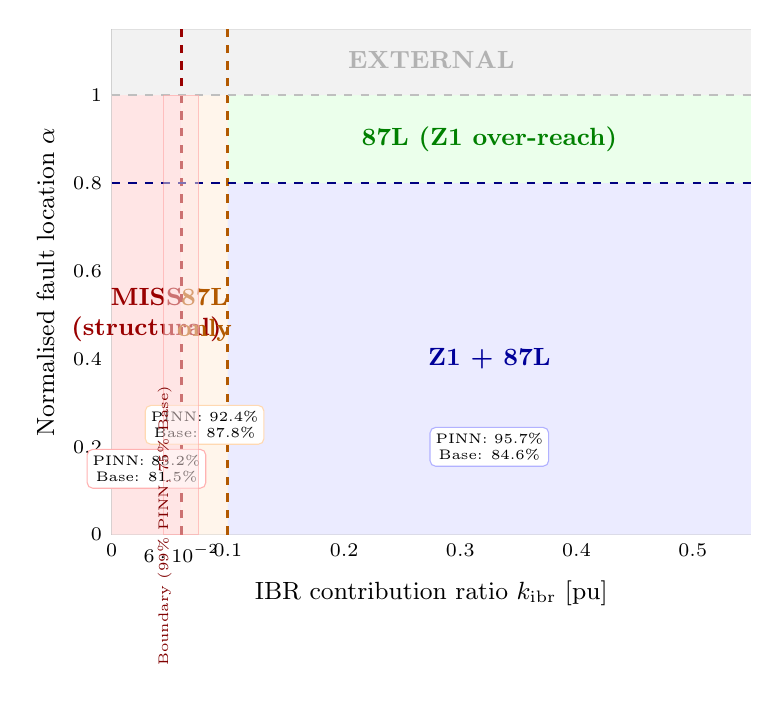
\begin{tikzpicture}
\begin{axis}[
  name         = bndax,
  width        = 0.80\textwidth,
  height       = 8.0cm,
  xlabel       = {IBR contribution ratio $k_\mathrm{ibr}$ [pu]},
  ylabel       = {Normalised fault location $\alpha$},
  xlabel style = {font=\small},
  ylabel style = {font=\small},
  xmin=0, xmax=0.55,
  ymin=0, ymax=1.15,
  xtick        = {0,0.06,0.10,0.20,0.30,0.40,0.50},
  ytick        = {0,0.2,0.4,0.6,0.8,1.0},
  xticklabel style={font=\scriptsize},
  yticklabel style={font=\scriptsize},
  tick style   = {draw=none},
  axis line style={gray!50},
  grid         = major,
  grid style   = {gray!10, dashed},
  clip=false,
]

%% Zone fills
% MISS zone: k < 0.06 (red-ish)
\addplot[red!15, fill=red!10, draw=none]
  coordinates {(0,0) (0.06,0) (0.06,1.0) (0,1.0)} \closedcycle;

% 87L-only zone: 0.06 ≤ k < 0.10
\addplot[orange!15, fill=orange!8, draw=none]
  coordinates {(0.06,0) (0.10,0) (0.10,1.0) (0.06,1.0)} \closedcycle;

% Z1 zone: k ≥ 0.10, alpha ≤ 0.80
\addplot[blue!15, fill=blue!8, draw=none]
  coordinates {(0.10,0) (0.55,0) (0.55,0.80) (0.10,0.80)} \closedcycle;

% 87L+Z1 zone: k ≥ 0.10, alpha > 0.80
\addplot[green!15, fill=green!8, draw=none]
  coordinates {(0.10,0.80) (0.55,0.80) (0.55,1.0) (0.10,1.0)} \closedcycle;

% EXT zone: alpha > 1.0
\addplot[gray!20, fill=gray!10, draw=none]
  coordinates {(0,1.0) (0.55,1.0) (0.55,1.15) (0,1.15)} \closedcycle;

%% Zone boundaries
\addplot[red!60!black, very thick, dashed]
  coordinates {(0.06,0) (0.06,1.15)};
\addplot[orange!70!black, very thick, dashed]
  coordinates {(0.10,0) (0.10,1.15)};
\addplot[blue!50!black, thick, dashed]
  coordinates {(0,0.80) (0.55,0.80)};
\addplot[gray!50, thick, dashed]
  coordinates {(0,1.0) (0.55,1.0)};

%% Zone labels
\node[red!60!black, font=\small\bfseries, align=center]
  at (axis cs:0.030, 0.50) {MISS\\(structural)};
\node[orange!70!black, font=\small\bfseries, align=center]
  at (axis cs:0.080, 0.50) {87L\\only};
\node[blue!60!black, font=\small\bfseries, align=center]
  at (axis cs:0.325, 0.40) {Z1 + 87L};
\node[green!50!black, font=\small\bfseries, align=center]
  at (axis cs:0.325, 0.90) {87L (Z1 over-reach)};
\node[gray!60, font=\small\bfseries]
  at (axis cs:0.275, 1.08) {EXTERNAL};

%% PINN accuracy annotations
\node[draw=blue!30, fill=white, rounded corners=2pt,
      font=\tiny, inner sep=2pt, align=center]
  at (axis cs:0.325, 0.20)
  {PINN: 95.7\%\\Base: 84.6\%};

\node[draw=orange!30, fill=white, rounded corners=2pt,
      font=\tiny, inner sep=2pt, align=center]
  at (axis cs:0.080, 0.25)
  {PINN: 92.4\%\\Base: 87.8\%};

\node[draw=red!30, fill=white, rounded corners=2pt,
      font=\tiny, inner sep=2pt, align=center]
  at (axis cs:0.030, 0.15)
  {PINN: 85.2\%\\Base: 81.5\%};

%% Boundary region highlight
\addplot[red!40, fill=red!10, opacity=0.5]
  coordinates {(0.045,0) (0.075,0) (0.075,1.0) (0.045,1.0)} \closedcycle;
\node[red!50!black, font=\tiny, rotate=90, anchor=south]
  at (axis cs:0.060, 0.02)
  {Boundary (99\% PINN, 75\% Base)};

\end{axis}
\end{tikzpicture}
}
  \caption{Protection decision zones in the ($k_\mathrm{ibr}$, $\alpha$) plane.
           Shading: MISS (red), 87L-only (orange), Z1+87L (blue), EXT (grey).
           Red highlight: threshold boundary $k\in[0.045,0.075]$.  PINN
           achieves 99\% accuracy in the boundary region vs 75\% for the
           baseline (+24\,pp), because physics constraint C1 enforces the
           correct label for $k<0.06$ regardless of measurement noise.}
  \label{fig:boundary}
\end{figure}

\noindent
The 24\,pp accuracy advantage in the boundary region is directly explained by
constraint C1.  When $k_\mathrm{ibr}=0.052$ (below threshold) with noise of
$\sigma_k=0.010$, approximately 30\% of samples will have a noisy
$k_\mathrm{est}>0.06$ and could be misclassified by a pure data-driven model.
The PINN's C1 residual penalises any non-MISS prediction in this region,
aligning the model with physics even when the noisy input crosses the threshold.

% ─────────────────────────────────────────────────────────────────────────────
\section{Summary}
\label{sec:summary}

\begin{enumerate}
  \item \textbf{Architecture}: 3-layer, 64-neuron PINN with three physics
    constraint residuals; $\lambda_\mathrm{phy}=0.20$; 12,676 parameters.

  \item \textbf{Accuracy}: 93.6\% overall (vs 85.8\% baseline); Z1 class
    improved by 11.2\,pp through quadrilateral boundary enforcement.

  \item \textbf{Violations}: 1.0\% physics violation rate vs 11.0\% baseline;
    91\% reduction attributable to constraint penalty.

  \item \textbf{Boundary}: 99\% accuracy at $k=0.06$ threshold (vs 75\%
    baseline); +24\,pp advantage from constraint C1.
\end{enumerate}

\noindent
TR-46 establishes the PINN classifier.  TR-47 develops the physics-constrained
feature engineering framework; TR-48 addresses online learning for changing
IBR fleets; TR-49 performs the ML integration study.

\bibliographystyle{IEEEtranN}
\bibliography{references46}

\end{document}
